\section{Visualisation}
%what are the features we want to emphasis?
%make a bullet list of something like that
Our goal is to design an interactive visualisation system on top of the structured prediction framework.
Figure~\ref{fig:overview} shows the overview of a live demo system, which consists of five major components: a map to display suggested routes, an input box for user query (upper left), a stacked score of routes (upper right), a POI list (lower left), and a radar chart to compare features of multiple POIs (lower right). 
The role and the construction of the four major components, besides the main map, are as follows:

%\begin{itemize}
\textbf{Query input}: A query consists of a starting POI and a trip length. 
Users can choose the starting POI by clicking icons on the map and can adjust the slide to set the trip length. 
In addition, three different travelling modes (e.g. bicycling, walking, and driving) are supported, 
and we optimise the suggested routes for each mode.

\textbf{Route score visualisation}: Ranks of candidate routes are determined by their total scores from the SSVM. 
The score of each route are decomposed into a set of scores for POIs and transitions along the route. 
We adopt the LineUp framework~\cite{gratzl2013lineup} designed to support the visualisation of multi-attribute ranking via stacked representation. 
To assist visualisation, both the POI and transition scores are properly scaled (see Appendix\footnote{https:arxiv.org/abs/???.????} for details).
Figure~\ref{fig:stack} shows the stacked bars of the top 10 scored routes, 
scores of different POI and transition are shown in different colours,
and the proportion of each bar indicates the importance of the corresponding POI and transition in the route.
At the left side, % of this representation,
the user can select one or more suggested routes to get the numerical scores of POIs and transitions.
All selected routes are drawn on the map, and the POIs in the most recent chosen route are shown with labelled icons.

\textbf{POI list}:
Users can select one or more suggested routes to get more detailed information. 
Specifically, information about the sequence of POIs in the selected route is provided, including POI names and their categories (e.g. Parks, Entertainment).
The POIs are ordered according to the suggested visiting order, with corresponding numerically labelled icons on the map.
The system also provides the estimated time and distance of the selected route at the top of this POI list.
When more than one route is selected, the system will display the POIs of the most recent chosen route.

\textbf{POI feature visualisation}: We further provide a radar chart to analyse the variation between POIs in a single route. 
For example, in Figure~\ref{fig:radar}, we compare two POIs, the \textit{Queen Victoria Market} and \textit{Melbourne Aquarium}, in terms of POI features and their importance in the suggested route. 
The radar chart shows the corresponding POI feature scores when a user selects a route.
In particular, the user can check/uncheck any POI in the selected route, and the feature scores of all checked POIs will be shown in the chart.
%\end{itemize}

\begin{figure}[t!]
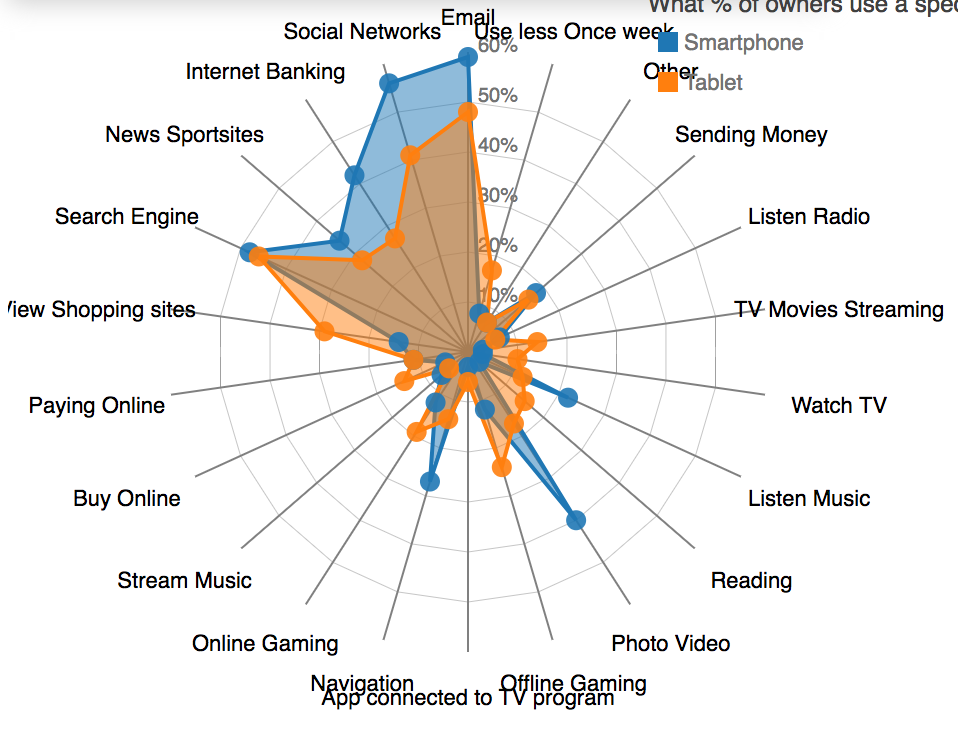
\includegraphics[width=0.6\linewidth]{figure/sample_radar.png} \vspace{-10pt}
    \caption{POI feature comparison between \textit{Melbourne Aquarium} and \textit{Queen Victoria Market}: the former scores higher on \textit{Popularity} and \textit{Visits difference} features whereas the latter scores higher on \textit{Visits} and \textit{Popularity difference} features.}
\label{fig:radar} \vspace{-1em}
\end{figure}
